\documentclass{article}
\usepackage[utf8]{inputenc}
\usepackage{amsmath}
\usepackage{fancyvrb}
\usepackage{array,multirow,graphicx}
\usepackage{float}
\usepackage{pdfpages}
\usepackage{lscape}
\addtolength{\topmargin}{-50pt}
\addtolength{\textheight}{100pt}

\title{Optimizing Hardware and Software for Gaussian Elimination
\large \\ Computer Systems Engineering (EDA332) Assignment}
\author{Oscar Dahlqvist}
\date{21-05-2021}

\begin{document}

\maketitle

\newpage
\tableofcontents

\setcounter{subsection}{0}
\newpage
\section{Introduction}
This assignment aims to produce hardware and software for a hypothetical company which demands a
cheap and fast microcomputer meant to handle Gaussian elimination efficiently. 
The mission of this report is to achieve the lowest Price*Performance number by writing optimised code for  available hardware components.

\section{The Assignment}
\subsection{Software}
Implement the elimination routine in MIPS assembler. Use single precision floating 
point instructions for all matrix computations. The program should run in the MIPS 
simulator MARS.
\subsection{Hardware}
Pick parts for a computer system considering both price and performance using the components in Appendix A. Performance is measured as the time it takes your program to triangularize a 24 × 24 reference matrix. 
Price is the sum of the component costs for processor, caches and memory. The goal 
is to minimize the product Price × Performance. The unit of this measure is µsC\$
(microSecondChalmersDollar)

\section{Development}
The final code and hardware setup can be found in Appendix \ref{sec:final_code}.
\subsection{Software}
The first step of software development was writing a slow implementation of the algorithm to make sure the it worked, a .c version of this implementation can be found in Appendix \ref{sec:gaussian_elim_c_code}.
\\\\
The second step was to always use pointers instead of array indexing since indexing is a demanding 
process with several calculations in comparison with pointers which require as little as a single add operation. Pointers keeping track of \verb!A[k][k], !\verb!A[k][j]!, \verb!A[i][k]! \& \verb!A[i][j]! were added. (\verb!AKK, AKJ, AIK, AIJ!)
Using indexing requires some thought since the code isn't only iterating right to left. Several registers needed to be used to store values which consider how the pointers should move after operations are performed on certain squares. Pseudo code for the pointer version van be found in Appendix \ref{sec:gaussian_elim_index_c_code}. 
\\\\
Several smaller optimizations were also made. Such as avoiding the slower floating point division and instead multiplying with \verb!1/A[k][k]! during the normalization and replacing all less than/greater than comparisons with equality checks and pre-calculating exactly where the last iteration step will end up. All stalls due to load-use and branch hazards were also removed by moving parts of the code, thankfully it is possible to remove all these hazards without adding any delay with this algorithm. 
\\\\
The trickiest optimization to do is to use the double loads/store operations of the floating point processor instead of loading each index separately. This could ideally half the number of iterations which needed to be done, at the cost of that each iteration would need take longer.
\\\\
However, this technique does cause several problems due to the fact that the doubles-store/load must be double aligned in memory. Another issue is that this technique will not work for odd matrices due to the following row sometimes being overwritten. While this somewhat could be prevented by stopping earlier and adding special cases this report hasn't done that since it would require more code slowing the program down and in practice the assignment was to optimize for a 24x24 matrix. But the code will still retain a copy the single word method which will be ran instead the program if supplied an odd matrix.
\\\\
It's relatively straightforward to implement double-store for the normalization loop (\verb!A[k][j] /= pivot!) by rounding the start of the iteration pointer down to the nearest double aligned address. This means that sometimes we will divide the pivot with itself, but as the pivot is set to 1.0 later regardless this is not a problem. The later subtraction loop is not much different. If rounded down just as the normalization it works. A[i][k] will end up overwritten half of the rows, but like the normalization, this is not a problem since A[i][k] is overwritten with 0 later.
\begin{figure}[h]
  \begin{minipage}{.45\linewidth}
    \centering
    $\begin{bmatrix}
      AKK & AKJ & .. & ..\\
      AIK & AIJ & .. & ..\\
      ..  & ..  & .. & ..\\
      ..  & ..  & .. & ..
    \end{bmatrix}$\\
    Step 1
  \end{minipage}
  \begin{minipage}{.45\linewidth}
    \centering
    $\begin{bmatrix}
      AKK & .. & AKJ & ..\\
      AIK & .. & AIJ & ..\\
      ..  & ..  & .. & ..\\
      ..  & ..  & .. & ..
    \end{bmatrix}$\\
    Step 2
  \end{minipage}
  \caption{How AIK and AKJ points during the single-store/load method}
\end{figure}
\begin{figure}[h]
  \begin{minipage}{.45\linewidth}
    \centering
    $\begin{bmatrix}
      AKK / AKJ & .. & .. & ..\\
      AIK / AIJ & .. & .. & ..\\
      ..  & ..  & .. & ..\\
      ..  & ..  & .. & ..
    \end{bmatrix}$\\Step 1
  \end{minipage}
  \begin{minipage}{.45\linewidth}
    \centering
    $\begin{bmatrix}
      AKK & .. & AKJ & ..\\
      AIK & .. & AIJ & ..\\
      ..  & ..  & .. & ..\\
      ..  & ..  & .. & ..
    \end{bmatrix}$\\
    Step 2
  \end{minipage}
  \caption{How AIK and AKJ points during the double-store/load method}
\end{figure}\\
Finally, instead of starting (AKJ,AIJ) at (AKK+4*, AIK+4) and rounding down it was faster to only add an alignment variable which toggles between 0 and 4. The toggling was made by xor-ing the variable with 4 for each k iteration.
\\\\
* 4 since the sizeof(float) = 4, hence adding 4 will point to the next element.

\subsection{Hardware}
The choice of simulated hardware mostly came after the code was written but small tweaks and previous versions were tested against each other to see which cycles count improves with which code. The choice of components matter not only to the price, caches also has a max frequency they can be ran at. The frequency of the slowest cache determines how fast we can clock the CPU, and hence how fast we can run the code. For the full specs available for each part check out Appendix \ref{sec:hardware_constaints}
\\\\
Regardless of version code with the best allowed hardware most of the execution time is spent on different types of stalling. The hardware choice matters a lot. Each part can give both positive and negative effects depending on the other hardware, say a faster frequency leads to the memory not being able to keep up. So while there are several areas of consider what fits the program testing a large sample of configurations is necessary to find the optimal.
\subsubsection{I-Cache}
Instruction cache misses is something you want to avoid at all costs and is very avoidable depending on how you code. The final main loop ended up 32 words, meaning it can be cached in it's entirety. Hence there is no need to have anything greater than the basic 32 word cache. That is, if the main loop is aligned to the cache blocks. Since if the main loop is not aligned it can't be fully cached, and performance will worsen. About a 2\% difference in my code (See table \ref{offest_table})
\begin{table}[h]
	\centering
	\begin{tabular}{|l|l|l|l|l|l|l|l|l|} \hline
        offset & 0 &	1 &	2 &	3 &	4 &	5 &	6 &	7 \\\hline
        cycles & 82958 &	82993 &	82993 &	83113 &	83113 &	81453 &	82958 &	82958 \\\hline
        misses & 1890 &	1925 &	1925 &	1925 &	1925 &	385 &	1890 &	1890 \\\hline
	\end{tabular}
	\caption{Effect of code alignment (for 8 word cache block size)}
	\label{offest_table}
\end{table}
\\
While the code could be made slightly faster with some loop unrolling this will result in more I-cache misses, which is a way bigger issue compared to the measly cycles that could be saved via loop unrolling. This could be combated with a larger cache, but the cost associated would mean you would need a ~10\% (very approximate number, depends on the rest of the hardware) performance increase to justify larger I-cache. To achieve better I-cache alignment extra NOP:s were added before the start of the function
\subsubsection{D-Cache}
The read and writes from the data memory are very spread out in the matrix which makes cache miss behaviour very unpredictable. Caching the whole Matrix is impossible with even the biggest cache so my approach was simply to test several combinations of cache sizes and configurations. All I know is that high associativity should be helpful.
\subsubsection{Memory/Write buffer}
It's not hard to make sure the write buffer usage is 100\% but if it won't reach 100\% even with a maxed size buffer you should increase the memory speed or the cache.
\\\\
Even though the memory access time is constant the cycle count to access memory wont due to the frequency of the cache.
\newpage
\section{Results}
\begin{table}[H]
	\centering
	\begin{tabular}{|l|l|l|l|l|l|l|l|l|l|l|} \hline
	    ~ & \multicolumn{3}{c|}{I-Cache} & \multicolumn{3}{c|}{D-Cache} & \multicolumn{4}{c|}{}
	    \\\hline
        mHz & type & a. & wb. & type & a. & wb. & mem & buf & cycles & \mu sC\$ \\\hline
		450	&	32A	&	1	&	8	&	64B	&	2	&	4	&	B	&	4	&	73925	&	553.61\\\hline
		450	&	32A	&	1	&	8	&	64B	&	2	&	4	&	B	&	4	&	105638	&	791.11\\\hline
		450	&	32A	&	1	&	8	&	64B	&	2	&	4	&	B	&	4	&	92324	&	691.40\\\hline
		450	&	32A	&	1	&	8	&	64B	&	2	&	4	&	B	&	4	&	91255	&	683.39\\\hline
		\hline
		475	&	32A	&	1	&	8	&	64A	&	1	&	4	&	B	&	4	&	104202	&	739.28\\\hline
		475	&	32A	&	1	&	8	&	64A	&	1	&	4	&	A	&	4	&	138214	&	835.10\\\hline
		450	&	32A	&	1	&	8	&	64B	&	2	&	4	&	B	&	4	&	83411	&	624.65\\\hline
		450	&	32A	&	1	&	8	&	64B	&	2	&	4	&	A	&	4	&	99310	&	633.37\\\hline
		425	&	32A	&	1	&	8	&	64C	&	4	&	4	&	B	&	4	&	82520	&	654.33\\\hline
		425	&	32A	&	1	&	8	&	64C	&	4	&	4	&	A	&	4	&	100866	&	681.14\\\hline
		\hline
		450	&	32A	&	1	&	8	&	64B	&	2	&	4	&	B	&	6	&	81163	&	618.64\\\hline
		450	&	32B	&	2	&	8	&	64B	&	2	&	4	&	B	&	6	&	81163	&	618.64\\\hline
		450	&	32C	&	4	&	8	&	64B	&	2	&	4	&	B	&	6	&	81163	&	618.64\\\hline
		\hline
		450	&	32A	&	1	&	8	&	128A	&	1	&	8	&	B	&	4	&	91310	&	734.53\\\hline
		425	&	32A	&	1	&	8	&	128B	&	2	&	8	&	B	&	4	&	93612	&	797.35\\\hline
		400	&	32A	&	1	&	8	&	128C	&	4	&	8	&	B	&	4	&	94424	&	854.53\\\hline
		450	&	32A	&	1	&	8	&	128A	&	1	&	4	&	B	&	4	&	89269	&	718.11\\\hline
		425	&	32A	&	1	&	8	&	128B	&	2	&	4	&	B	&	4	&	79868	&	680.28\\\hline
		400	&	32A	&	1	&	8	&	128C	&	4	&	4	&	B	&	4	&	80006	&	724.05\\\hline
		\hline
		500	&	32A	&	1	&	8	&	32A	&	1	&	8	&	B	&	8	&	172395	&	1117.11\\\hline
		475	&	32A	&	1	&	8	&	32B	&	2	&	8	&	B	&	8	&	135922	&	927.13\\\hline
		450	&	32A	&	1	&	8	&	32C	&	4	&	8	&	B	&	8	&	124236	&	894.49\\\hline
		500	&	32A	&	1	&	8	&	32A	&	1	&	4	&	B	&	8	&	126276	&	818.26\\\hline
		475	&	32A	&	1	&	8	&	32B	&	2	&	4	&	B	&	8	&	108570	&	740.56\\\hline
		450	&	32A	&	1	&	8	&	32C	&	4	&	4	&	B	&	8	&	109456	&	788.08\\\hline
		500	&	32A	&	1	&	8	&	32A	&	1	&	2	&	B	&	8	&	129078	&	836.42\\\hline
		475	&	32A	&	1	&	8	&	32B	&	2	&	2	&	B	&	8	&	123337	&	841.28\\\hline
		450	&	32A	&	1	&	8	&	32C	&	4	&	2	&	B	&	8	&	122982	&	885.47\\\hline
		\hline
		475	&	32A	&	1	&	8	&	64A	&	1	&	4	&	B	&	4	&	104911	&	744.31\\\hline
		450	&	32A	&	1	&	8	&	64B	&	2	&	4	&	B	&	4	&	83411	&	624.65\\\hline
		425	&	32A	&	1	&	8	&	64C	&	4	&	4	&	B	&	4	&	82170	&	651.55\\\hline
		\hline
		450	&	32A	&	1	&	8	&	64B	&	2	&	4	&	B	&	4	&	83411	&	624.65\\\hline
		450	&	32A	&	1	&	8	&	64B	&	2	&	4	&	B	&	5	&	81453	&	615.42\\\hline
		450	&	32A	&	1	&	8	&	64B	&	2	&	4	&	B	&	6	&	81163	&	618.64\\\hline
		450	&	32A	&	1	&	8	&	64B	&	2	&	4	&	B	&	7	&	80849	&	621.63\\\hline
		450	&	32A	&	1	&	8	&	64B	&	2	&	4	&	B	&	8	&	80505	&	624.36\\\hline
		450	&	32A	&	1	&	8	&	64B	&	2	&	4	&	B	&	9	&	80370	&	628.67\\\hline
		\end{tabular}
	\caption{Table of runs, a. = associativty, wb. = words/block \\
	For table with complete statistics see Appendix \ref{sec:full_stats}}
	\label{offest_table}
\end{table}

\newpage
\section{Conclusion}
The best hardware configuration found is:
\begin{description}
    \item[CPU] The CPU clocked 450mHz due to the D-Cache speed for 2C\$.
    \item[I-Cache] Any 32 word cache works for 0C\$.
    \item[D-Cache] 64 words of 2 way associative cache with 16 blocks with 4 words for each block for 0.25C\$.
    \item[Memory] The faster memory (B) for 0.5C\$.
    \item[Write Buffer] 5 bytes of buffer for 0.15C\$.
\end{description}
\begin{figure}[h]
    \begin{minipage}{.79\linewidth}
        \centering
        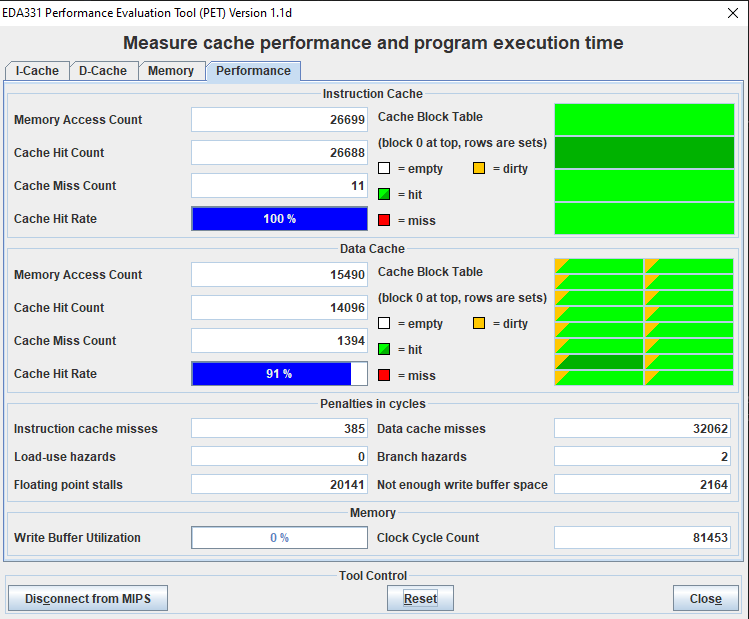
\includegraphics[scale=.4]{stats.png}
	    \caption{Program breakdown from MARS}
	\end{minipage}
    \begin{minipage}{.2\linewidth}
        \centering
        \begin{tabular}{|l|l|} \hline
            Cycles & 81453 \\\hline
            Time (\mu s) & 181.01 \\\hline
            Price (C\$) & 3.4 \\\hline
            \mu sC\$  & 615.42 \\\hline
	    \end{tabular}
        \centering
	    \caption{\\Stats of optimal solution}
	\end{minipage}
\end{figure}

\subsection{Improvement Ideas}
\begin{description}
    \item[More Cases] Another double-store algorithm could be implemented for odd matrices
    \item[Use more cache effective algorithm] The biggest percent of stalling is caused by D-Cache misses, if one were to use and algorithm which only accesses limited parts of the matrix at a time instead of all over this could greatly be reduced.
    \item[Use a better algorithm in general] Better algorithms exist, but that a task for another day and another course.
\end{description}



\newpage

\renewcommand\thesection{\Alph{section}}
\setcounter{section}{0}
\section{Hardware Constraints}
\label{sec:hardware_constaints}

\subsection{Processor}
The base hardware is a computer system consists of a MIPS-compatible microprocessor with five pipeline 
stages and delayed branching. There are also two coprocessors, one for memory 
management and exception handling and one for floating point 
arithmetic operations.
The CPU operates at a clock frequency of 500 MHz and its price is 2C\$. 
\subsection{Caches}
The memory system includes separate instruction and data caches. The block 
replacement policy is Least Recently Used (LRU) and the write policy is Write Back. 
Cache size, block size and associativity are 
configurable parameters and they can be set differently for the two caches. Available 
configurations are given in table \ref{cache_table}.
\begin{table}[h]
	\centering
	\begin{tabular}{|l|l|l|l|l|} \hline
        Name & Cache Size & Associativity & Max Clock Frequency & Extra Cost        \\ \hline\hline
        32A &32	& 1	& 500	& 0        \\ \hline
        32B &32	& 2	& 475	& 0        \\ \hline
        32C &32	& 4	& 450	& 0        \\ \hline
        64A &64	& 1	& 475	& 0.25        \\ \hline
        64B &64	& 2	& 450	& 0.25        \\ \hline
        64C &64	& 4	& 425	& 0.25        \\ \hline
        128A &128	& 1	& 450	& 0.5        \\ \hline
        128B &128	& 2	& 425	& 0.5        \\ \hline
        128C &128	& 4	& 400	& 0.5        \\ \hline
	\end{tabular}
	\caption{Available Caches}
	\label{cache_table}
\end{table}
\subsubsection{Write Buffer}
The data cache has an optional write buffer of variable size to reduce the number of 
stall cycles due to memory writes. 
The cost of buffer space is 0.03 C\$/word. You are allowed to use a write buffer of up 
to 12 words, or none at all



\subsection{Memory}
There are two types of memory modules to choose from. Table \ref{memory_table} lists their 
costs and their latencies for the first word as well as for other words that are accessed 
from a block. 
\begin{table}[H]
	\centering
	\begin{tabular}{|l|l|l|l|} \hline
        Type & $1_{st}$ word access time (ns) & Access time, other words (ns) & Cost (C\$) \\ \hline\hline
        A	& 44	& 8	& 0.5        \\ \hline
        B	& 30	& 6	& 1.0        \\ \hline
	\end{tabular}
	\caption{Available Memory}
	\label{memory_table}
\end{table}

\newpage
\section{Simple Gaussian Elimination}
\label{sec:gaussian_elim_c_code}
\begin{verbatim}
/* reduce matrix A to upper triangular form */
void eliminate (double **A, int N) { 
    int i, j, k; 
    /* loop over all diagonal (pivot) elements */ 
    for (k = 0; k < N; k++) { 
        /* for all elements in pivot row right of pivot element */ 
        for (j = k + 1; j < N; j++) { //Normalize row
            /* divide by pivot element */
            A[k][j] = A[k][j] / A[k][k];
        } 
        /* set pivot element to 1.0 */
        A[k][k] = 1.0; 
        /* for all elements below pivot row right of pivot column */ 
        for (i = k + 1; i < N; i++) { // Subtract row k from others
            for (j = k + 1; j < N; j++) {
                A[i][j] = A[i][j] - A[i][k] * A[k][j];
            }
            A[i][k] = 0.0; 
        }
    } /* end pivot loop */
} /* end eliminate *
\end{verbatim}

\newpage
\section{Gaussian elimination using pointers}
\label{sec:gaussian_elim_index_c_code}
\begin{verbatim}
void eliminate (double **A, int N) { 
    float* ak, akk, aik, akj, aij
    float* akjMax, aikMax, akMax, matrixEnd
    int rowSize, akkStep
    
    rowSize = N * sizeof(float)
    akkStep = rowSize + sizeof(float)
    
    ak = A
    akk = A
    matrixEnd = A+N*N*sizeof(float)
    akMax = matrixEnd - rowSize
    
    aikMax = matrixEnd
    
    do {
        akj = ak+rowSize
        do {
            akj -= sizeof(float)
            *akj /= *akk
        } while (akj != akk)

        *akk = 1
        
        aik = akk+rowSize
        akjMax = ak+rowSize
        
        do {
            aij = aik + 4
            akj = akk + 4
            do {
                *aij = *aij - *aik * *akj
                aij += sizeof(float)
                akj += sizeof(float)
            } while (akj != akjMax)
            *aik = 0.0f
            aik += rowSize
        } while (aik != aikMax)
            
        aik_max += sizeof(float)
        ak += sizeof(float)
        akk += akkStep
    } while (ak != akMax)
}
\end{verbatim}

\newpage
\section{Extended Test Results}
\label{sec:full_stats}
\begin{figure}[H]
    \includepdf[page={1},angle=-90,origin=c, scale=0.8]{x_runs.pdf}
\end{figure}

\newpage
\tiny
\section{Final Code}
\label{sec:final_code}
\begin{verbatim}
### Text segment
        .text
start:
        la      $a0, matrix_24x24       # a0 = A (base address of matrix)
        li      $a1, 24             # a1 = N (number of elements per row)
        
        jal     eliminate
        nop
        jal     exit
        
        la      $a0, matrix_4x4     # a0 = A (base address of matrix)
        li      $a1, 4              # a1 = N (number of elements per row)
                                    # <debug>
        jal     print_matrix        # print matrix before elimination
        nop                         # </debug>
        jal     eliminate           # triangularize matrix!
        nop                         # <debug>
        jal     print_matrix        # print matrix after elimination
        nop                         # </debug>
        jal     exit

exit:
        li      $v0, 10             # specify exit system call
        syscall                     # exit program

################################################################################
# eliminate - Triangularize matrix.
#
# Args:     $a0  - base address of matrix (A)
#           $a1  - number of elements per row (N)
# <aliases>
.eqv A          $a0
.eqv N          $a1

.eqv CON1F      $f0 # for storing 1.0f
.eqv TMPF       $f1 # temp float register
.eqv AKK_iV     $f2 # 1/A[K][K]
.eqv AIK_V      $f3 # Not used at the same time as AKK_iV, so nothing will be overwiden

.eqv AIJ_V      $f4
.eqv AIJ_V2     $f5 
.eqv AKJ_V      $f6
.eqv AKJ_V2     $f7
                    # The register aliases of the following paragrph derives from the naive v1 implementation
.eqv NXTRW      $t1 # points to the first item in the row after the current one being processed
.eqv AKK        $t2 # points to the &A[k][k] during doWhile_k
.eqv AKJ        $t3 # points to the &A[k][j] during doWhile_akj and doWhile_i
.eqv AIJ        $t4 # points to the &A[i][j] during doWhile_i 
.eqv AIK        $t5 # points to the &A[i][k] during doWhile_i
.eqv AIK_MAX    $t6 # AKJ_MAX != AKJ could be replaced with AKJ < AKJ_MAX, but I can use != since i know the increment steps (lt/gt check is slower)
#.eqv AKJ_MAX   $t7 # AIK_MAX != AIK could be replaced with AIK < AIK_MAX, -||-

.eqv RWSIZE     $t8 # the number of bytes in a matrix row
.eqv AKKSTEP    $t9 # the number of bytes you must offset to reach the (1 right, 1 down) diagonal from a given space
.eqv MATRIXEND  $v0 # the first memory adress after the matrix
.eqv ALIGN      $v1 # 
# </aliases>
nop
nop # Padding to get the best
nop # I-Cache allignment
nop # added last of everything
nop
eliminate:
        #<setup>
        sll RWSIZE, N, 2                # RWSIZE = N*4 = N*sizeof(float)
        lwc1 CON1F, float1.0            # CON1F = 1.0f
        addiu AKKSTEP, RWSIZE, 4        # AKKSTEP = RWSIZE + sizeof(float)
        
        move AKK, A                     # AKK = A[0][0]
        add NXTRW, A, RWSIZE            # NXTRW = &A[1][0]
        mul $t0, N, N                   # t0 = N*N = number of cells in matrix
        sll $t0, $t0, 2                 # t0 = t0*4 = t0*sizeof(float) = number of bytes in matrix
        addu AIK_MAX, A, $t0            #AIK_MAX = &A[N][0] 
        move MATRIXEND, AIK_MAX         #MATRIXEND = &A[N][0]
        #</setup>
        
        andi $t0, N, 1                  #t0 = 1 if N is odd
        beq $t0, 1, eliminate_slow      
        andi $t0, A, 4                  #t0 = 4 if not double alligned
        beq $t0, 4, eliminate_slow

eliminate_alligned_even:
        andi ALIGN, A, 4
elim_k:         
            lwc1 TMPF, 0(AKK)
            add AKJ, AKK, ALIGN         # start iterating from A[K][K+1] or A[K][K] depending on allign
            div.s AKK_iV, CON1F, TMPF   # AKK_iv = 1/A[K][K], Some precition is lost here
elim_akj:
                ldc1 AKJ_V, 0(AKJ)          # tmp = A[K][J]
                addiu AKJ, AKJ, 8           # AKJ += sizeof(float)*2
                mul.s AKJ_V, AKJ_V, AKK_iV  # A[K][J] = A[K][J] / A[K][K]
                mul.s AKJ_V2, AKJ_V2, AKK_iV# A[K][J+1] = A[K][J+1] / A[K][K]
elim_akj_CMP:
                bne AKJ, NXTRW, elim_akj
                sdc1 AKJ_V, -8(AKJ)         # A[K][J] = TMPF = A[K][J] / A[K][K]
                                            #  -8 offset since AKJ has already been increased
                                            
            swc1 CON1F, 0(AKK)          # unneccesary half of the time but it's slower to check for it      
            addu AIK, AKK, RWSIZE       # AIK = AKK + RWSIZE (down 1 from AKK)  
            
elim_i:     
                lwc1 AIK_V, 0(AIK)
                
                addu AIJ, AIK, ALIGN        # the ALIGN means that we sometimes add 4 to the starting point of the iteration to ensure doubleword alignment.
                addu AKJ, AKK, ALIGN        #  however, when 4 isn't added it means M[AIK] will be overwritten by the first iteration of elim_j
                                            #  this is not a problem however since we alread fetched the correct AIK_V before writing garbage
                                            #  and M[AIK] is overwritten with 0 afterwards              
elim_j:     
                    ldc1 AKJ_V, 0(AKJ)  
                    ldc1 AIJ_V, 0(AIJ)              
                    mul.s TMPF, AIK_V, AKJ_V        # tmp = A[i][k] x A[k][j]
                    sub.s AIJ_V, AIJ_V, TMPF        # A[i][j] -= tmp
                    mul.s TMPF, AIK_V, AKJ_V2       # tmp = A[i][k] x A[k][j+1]
                    sub.s AIJ_V2, AIJ_V2, TMPF      # A[i][j+1] -= tmp
                    
                    addiu AKJ, AKJ, 8               # AKJ += sizeof(float)*2
                    
                    sdc1 AIJ_V, 0(AIJ)              # A[i][j] = A[i][j] - A[i][k] * A[k][j]
                                                    # A[i][j+1] = A[i][j+1] - A[i][k] * A[k][j+1]
        
elim_j_CMP:         bne AKJ, NXTRW, elim_j      # if AKJ overflowed to the next (aka wrong) row stop looping
                    addiu AIJ, AIJ, 8           # AIJ += sizeof(float)*2
                
                sw $0, 0(AIK)                   # no need for coproc1 operations here since 0.0f = 0x0
elim_i_CMP:     bne AIK, AIK_MAX, elim_i        # if AIK is outside the matrix (only checks at A[N][k] to improve efficiency)
                addu AIK, AIK, RWSIZE           # AIK += RWSIZE (move AIK one space down)
            
            xori ALIGN, ALIGN, 4            # Every other line can not have 4 added (or doubleword will not be alligned)
            
            addu NXTRW, NXTRW, RWSIZE       # NXTRW += RWSIZE (1 down)
            addiu AIK_MAX, AIK_MAX, 4       # AIK_MAX += sizeof(float)
elim_k_CMP: 
            bne NXTRW, MATRIXEND, elim_k    # no code need to be ran for the last row since we know it must be 0 .. 0 1 (as we assume the matrix is invertible)
            addu AKK, AKK, AKKSTEP          # AKK += AKKSTEP (right 1, down 1 from AKK)
            
        subu $t0, MATRIXEND, 4          # t0 <- adress of last item in matrix (bottom right)
        
        jr   $ra                        # return from subroutine
        swc1 CON1F, 0($t0)              # set last item in matrix to 1.0f

################################################################################
eliminate_slow:
elim2_k:            
            lwc1 TMPF, 0(AKK)
            add AKJ, AKK, 4             # start iterating from A[K][K+1]
            div.s AKK_iV, CON1F, TMPF   # AKK_iv = 1/A[K][K], Some precition is lost here
elim2_akj:
                lwc1 AKJ_V, 0(AKJ)          # tmp = A[K][J]
                addiu AKJ, AKJ, 4           # AKJ += sizeof(float)
                mul.s AKJ_V, AKJ_V, AKK_iV  # A[K][J] = A[K][J] / A[K][K]
elim2_akj_CMP:
                bne AKJ, NXTRW, elim2_akj
                swc1 AKJ_V, -4(AKJ)         # A[K][J] = TMPF = A[K][J] / A[K][K]
                                            #  -4 offset since AKJ has already been increased
            swc1 CON1F, 0(AKK)
            
            addu AIK, AKK, RWSIZE       # AIK = AKK + RWSIZE (down 1 from AKK)  
            
elim2_i:        
                lwc1 AIK_V, 0(AIK)
                
                addiu AIJ, AIK, 4
                addiu AKJ, AKK, 4
                sw $0, 0(AIK)               
elim2_j:        
                    lwc1 AKJ_V, 0(AKJ)  
                    lwc1 AIJ_V, 0(AIJ)              
                    mul.s TMPF, AIK_V, AKJ_V        # tmp = A[i][k] x A[k][j]
                    sub.s AIJ_V, AIJ_V, TMPF        # A[i][j] -= tmp                    
                    addiu AKJ, AKJ, 4               # AKJ += sizeof(float)              
                    swc1 AIJ_V, 0(AIJ)              # A[i][j] = A[i][j] - A[i][k] * A[k][j]
        
elim2_j_CMP:        bne AKJ, NXTRW, elim2_j     # if AKJ overflowed to the next (aka wrong) row stop looping
                    addiu AIJ, AIJ, 4           # AIJ += sizeof(float)
                
elim2_i_CMP:    bne AIK, AIK_MAX, elim2_i       # if AIK is outside the matrix (only checks at A[N][k] to improve efficiency)
                addu AIK, AIK, RWSIZE           # AIK += RWSIZE (move AIK one space down)
            
            addu NXTRW, NXTRW, RWSIZE       # NXTRW += RWSIZE (1 down)
            addiu AIK_MAX, AIK_MAX, 4       # AIK_MAX += sizeof(float)
elim2_k_CMP:    
            bne NXTRW, MATRIXEND, elim2_k   # no code need to be ran for the last row since we know it must be 0 .. 0 1 (as we assume the matrix is invertible)
            addu AKK, AKK, AKKSTEP          # AKK += AKKSTEP (right 1, down 1 from AKK)
            
        subu $t0, MATRIXEND, 4          # t0 <- adress of last item in matrix (bottom right)
        jr   $ra
        swc1 CON1F, 0($t0)              # set last item in matrix to 1.0f
        
################################################################################
# getElem - Get address and content of matrix element A[a][b].
#
# Argument registers $a0..$a3 are preserved across calls
#
# Args:     $a0  - base address of matrix (A)
#           $a1  - number of elements per row (N)
#           $a2  - row number (a)
#           $a3  - column number (b)
#                       
# Returns:  $v0  - Address to A[a][b]
#           $f0  - Contents of A[a][b] (single precision)
getElem:
        addiu   $sp, $sp, -12       # allocate stack frame
        sw      $s2, 8($sp)
        sw      $s1, 4($sp)
        sw      $s0, 0($sp)         # done saving registers
        
        sll     $s2, $a1, 2         # s2 = 4*N (number of bytes per row)
        multu   $a2, $s2            # result will be 32-bit unless the matrix is huge
        mflo    $s1                 # s1 = a*s2
        addu    $s1, $s1, $a0       # Now s1 contains address to row a
        sll     $s0, $a3, 2         # s0 = 4*b (byte offset of column b)
        addu    $v0, $s1, $s0       # Now we have address to A[a][b] in v0...
        l.s     $f0, 0($v0)         # ... and contents of A[a][b] in f0.
        
        lw      $s2, 8($sp)
        lw      $s1, 4($sp)
        lw      $s0, 0($sp)         # done restoring registers
        addiu   $sp, $sp, 12        # remove stack frame
        
        jr      $ra                 # return from subroutine
        nop                         # this is the delay slot associated with all types of jumps

################################################################################
# print_matrix
#
# This routine is for debugging purposes only. 
# Do not call this routine when timing your code!
#
# print_matrix uses floating point register $f12.
# the value of $f12 is _not_ preserved across calls.
#
# Args:     $a0  - base address of matrix (A)
#           $a1  - number of elements per row (N) 
print_matrix:
        addiu   $sp,  $sp, -20      # allocate stack frame
        sw      $ra,  16($sp)
        sw      $s2,  12($sp)
        sw      $s1,  8($sp)
        sw      $s0,  4($sp) 
        sw      $a0,  0($sp)        # done saving registers

        move    $s2,  $a0           # s2 = a0 (array pointer)
        move    $s1,  $zero         # s1 = 0  (row index)
loop_s1:
        move    $s0,  $zero         # s0 = 0  (column index)
loop_s0:
        l.s     $f12, 0($s2)        # $f12 = A[s1][s0]
        li      $v0,  2             # specify print float system call
        syscall                     # print A[s1][s0]
        la      $a0,  spaces
        li      $v0,  4             # specify print string system call
        syscall                     # print spaces

        addiu   $s2,  $s2, 4        # increment pointer by 4

        addiu   $s0,  $s0, 1        # increment s0
        blt     $s0,  $a1, loop_s0  # loop while s0 < a1
        nop
        la      $a0,  newline
        syscall                     # print newline
        addiu   $s1,  $s1, 1        # increment s1
        blt     $s1,  $a1, loop_s1  # loop while s1 < a1
        nop
        la      $a0,  newline
        syscall                     # print newline

        lw      $ra,  16($sp)
        lw      $s2,  12($sp)
        lw      $s1,  8($sp)
        lw      $s0,  4($sp)
        lw      $a0,  0($sp)        # done restoring registers
        addiu   $sp,  $sp, 20       # remove stack frame

        jr      $ra                 # return from subroutine
        nop                         # this is the delay slot associated with all types of jumps

### End of text segment

### Data segment 
        .data
        
### String constants
spaces:
        .asciiz "   "               # spaces to insert between numbers
newline:
        .asciiz "\n"                # newline

### Float constants
float1.0:
        .float 1.0(4x4) ##
....

\end{verbatim}



\end{document}
